% ============================================================
%  CSE200 Online-1 (C2)  ->  "The Solar System"
%  Assets in this folder: sun.png mercury.png venus.png earth.png mars.png
%                         jupiter.png saturn.png uranus.png neptune.png
%                         solar_system.bib
%  Compile:  pdflatex Q5_SolarSystem.tex   (twice, for TOC + cross-references)
% ============================================================
\documentclass[11pt]{article}

\usepackage[T1]{fontenc}
\usepackage[utf8]{inputenc}
\usepackage[margin=1in]{geometry}
\usepackage{amsmath}
\usepackage{amssymb}
\usepackage{mathtools}
\usepackage{graphicx}
\usepackage{subcaption}
\usepackage{xcolor}
\usepackage[table]{xcolor}
\usepackage{multirow}
\usepackage{array}
\usepackage{enumitem}
\usepackage{amsthm}          % proposition + proof
\usepackage{hyperref}

\definecolor{tocblue}{RGB}{40,90,160}
\hypersetup{colorlinks=true, linkcolor=black, citecolor=black, urlcolor=blue}

% colour only the word "Contents"
\renewcommand{\contentsname}{\textcolor{tocblue}{Contents}}

% Proposition environment numbered within sections -> "Proposition 3.1"
\newtheorem{proposition}{Proposition}[section]

\title{\textsc{\LARGE The Solar System}}
\author{Johannes Kepler\textsuperscript{1}\\[0.5em]
        {\small \textsuperscript{1}Imperial Mathematician, Prague}}
\date{}

\begin{document}
\maketitle
\thispagestyle{empty}

\tableofcontents
\newpage

% ------------------------------------------------------------
\section{Our Planetary Neighborhood}

\subsection{The Sun and Its Planets}
The Sun and its gravity-bound bodies form the Solar System~\cite{kepler1609}. See
\href{https://science.nasa.gov/solar-system/}{NASA Solar System Exploration}. In
increasing distance, the planets are
\begin{quote}
    Mercury, Venus, Earth, Mars, Jupiter, Saturn, Uranus, Neptune.
\end{quote}
The planets form two groups:
\begin{enumerate}[label=(\Roman*)]
    \item \textbf{Inner planets}
        \begin{itemize}[label=$\dagger$]
            \item Mercury, Venus, Earth, and Mars belong to this group.
            \item They are comparatively small and have solid surfaces.
            \item They are also called the terrestrial planets.
        \end{itemize}
    \item \textbf{Outer planets}
        \begin{itemize}[label=$\dagger$]
            \item Jupiter and Saturn are gas giants.
            \item Uranus and Neptune are commonly called ice giants.
            \item All four outer planets possess ring systems.
        \end{itemize}
\end{enumerate}

\textcolor{blue}{The inner planets are small, dense, and relatively close to the
Sun,} whereas \textcolor{red}{the outer planets are much larger and travel along
considerably wider orbits.}

\subsection{Portraits of the Solar System}
Figure~\ref{fig:solar} shows the Sun and eight planets.\footnote{Sizes and
distances are schematic.}
Compare Mars in Figure~\ref{fig:mars} with Jupiter in Figure~\ref{fig:jupiter}.

\begin{figure}[ht]
    \centering
    {\large\textbf{Star}}\par\medskip
    \begin{subfigure}{0.30\textwidth}
        \centering
        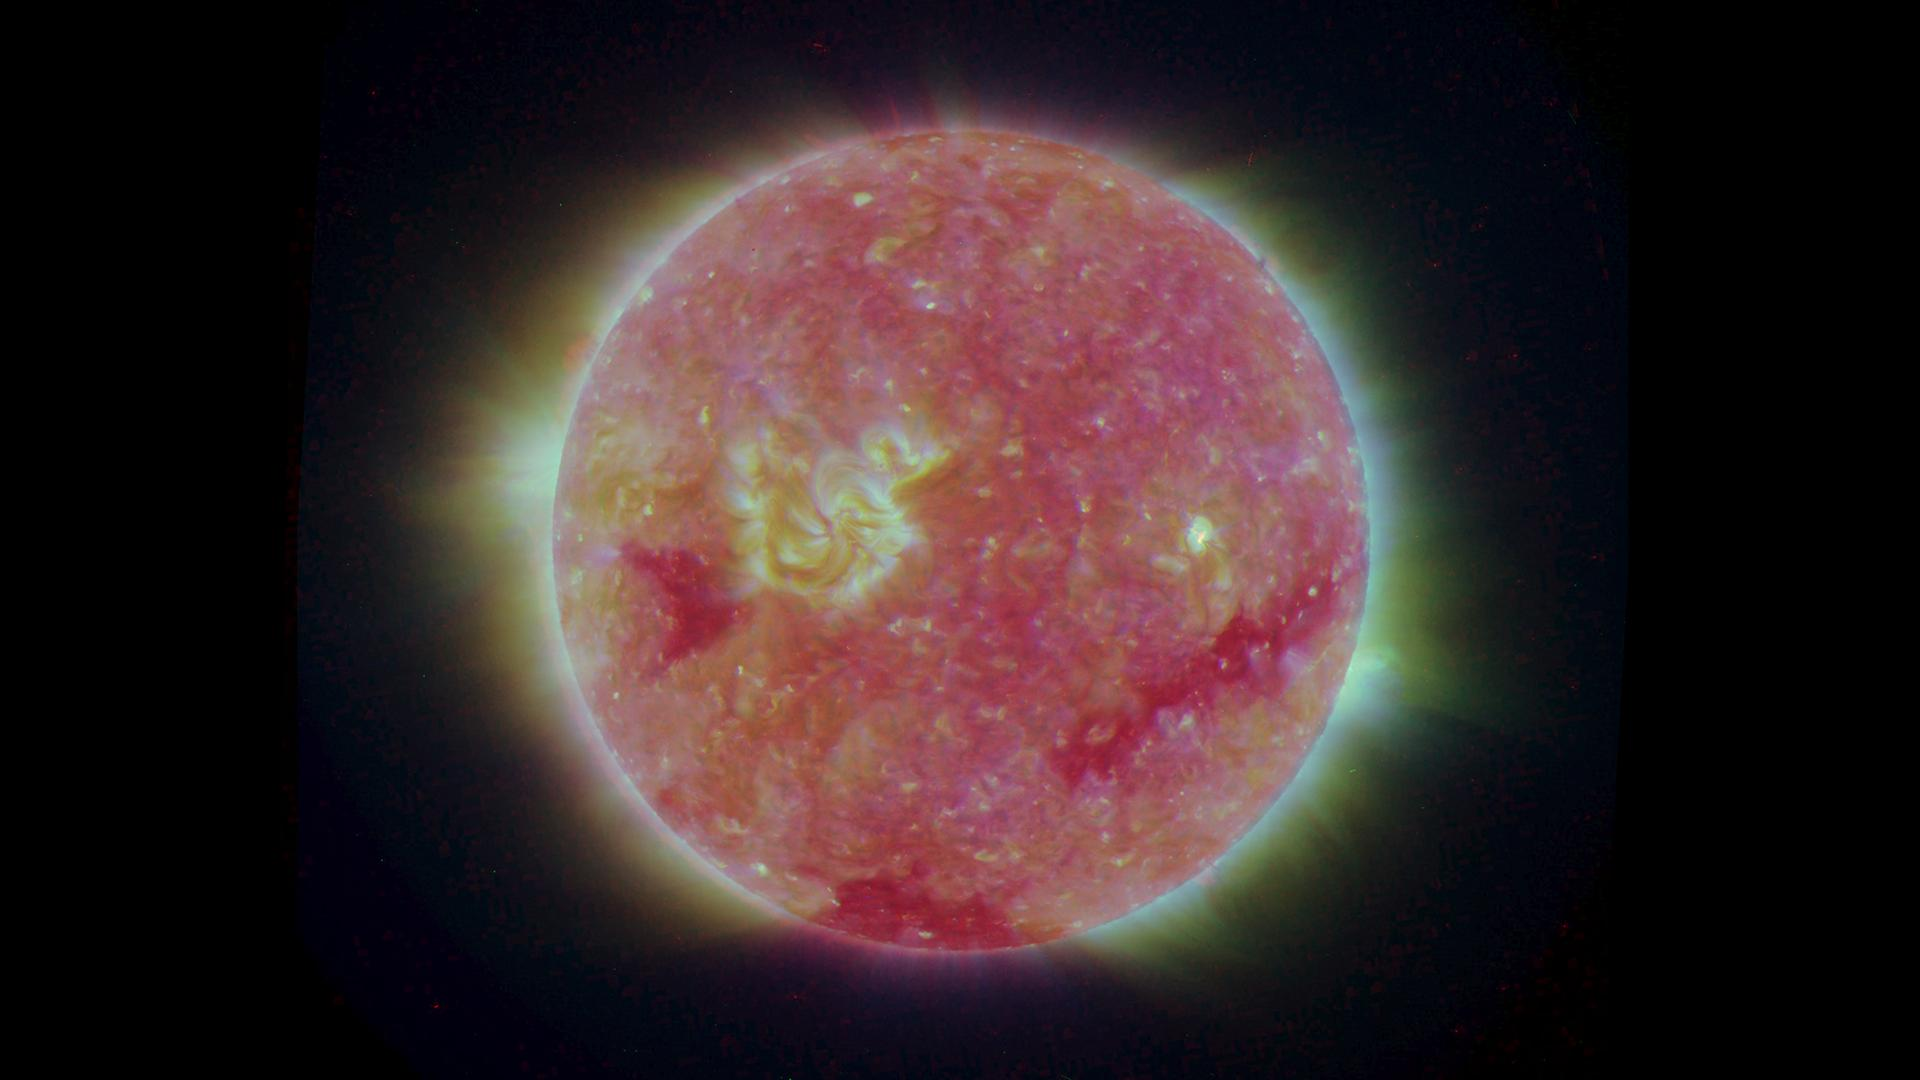
\includegraphics[width=0.6\textwidth]{sun.png}
        \caption{The Sun}
    \end{subfigure}

    \bigskip
    {\large\textbf{Inner Planets}}\par\medskip
    \begin{subfigure}{0.22\textwidth}\centering
        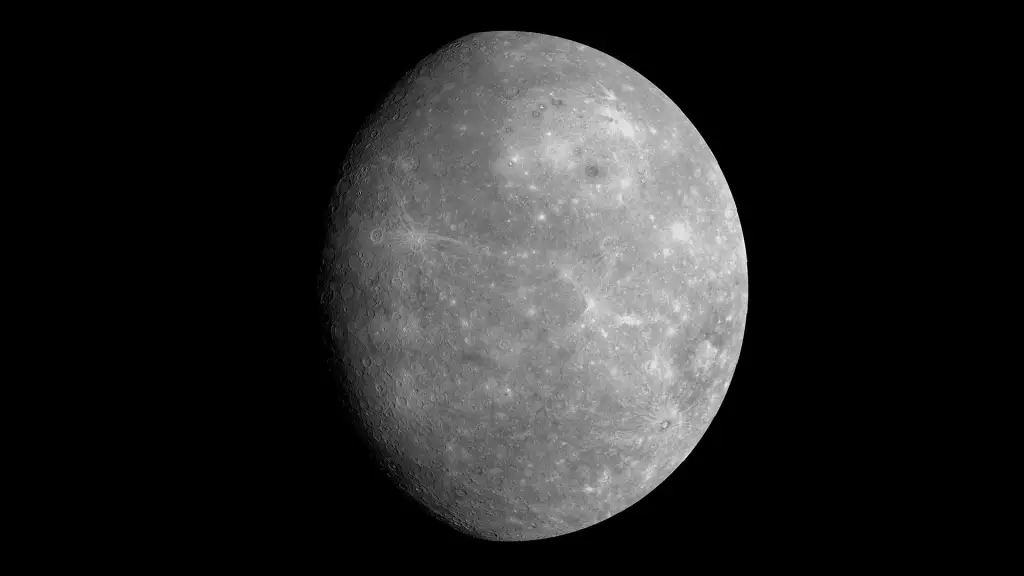
\includegraphics[width=\textwidth]{mercury.png}\caption{Mercury}\end{subfigure}\hfill
    \begin{subfigure}{0.22\textwidth}\centering
        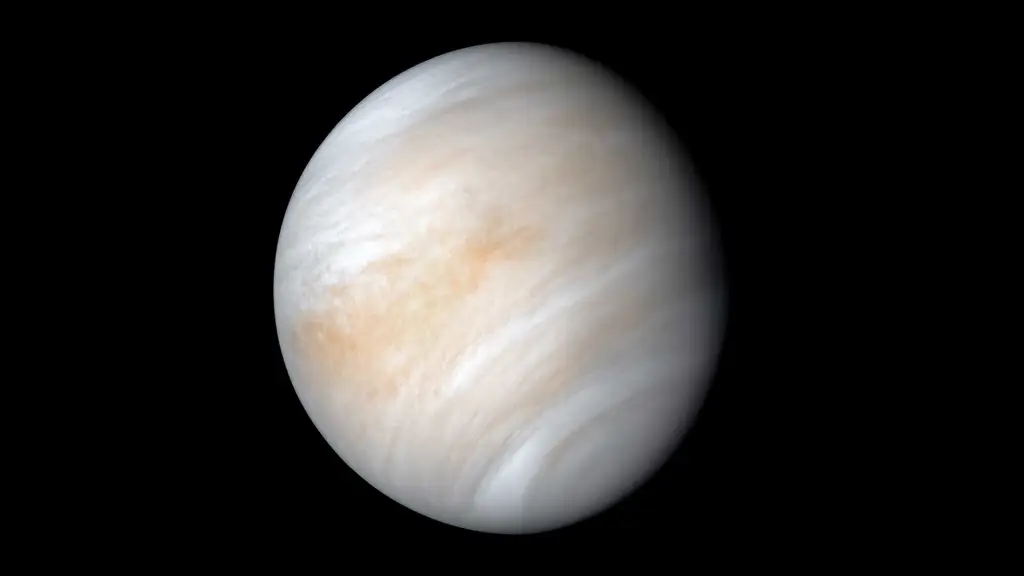
\includegraphics[width=\textwidth]{venus.png}\caption{Venus}\end{subfigure}\hfill
    \begin{subfigure}{0.22\textwidth}\centering
        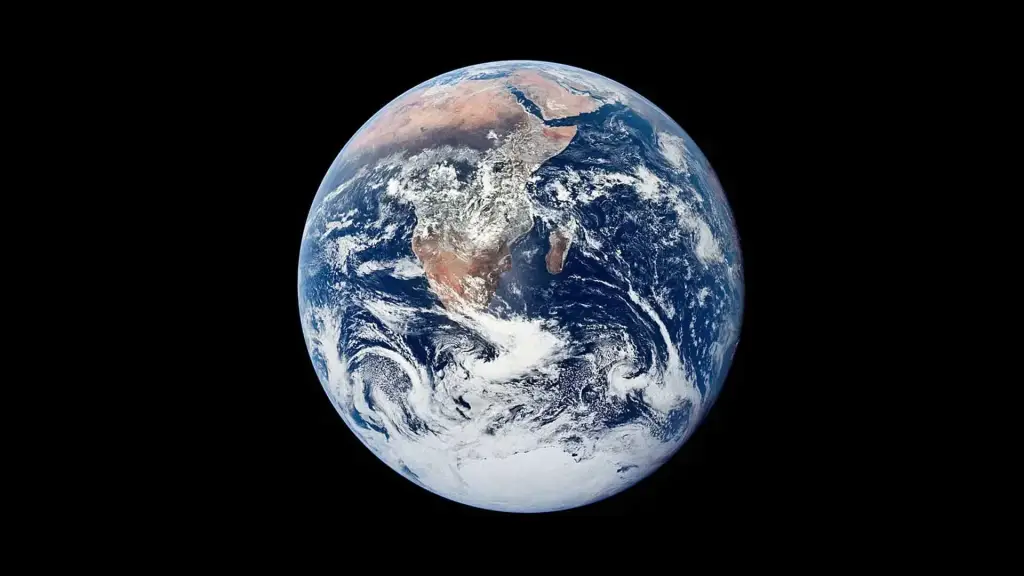
\includegraphics[width=\textwidth]{earth.png}\caption{Earth}\end{subfigure}\hfill
    \begin{subfigure}{0.22\textwidth}\centering
        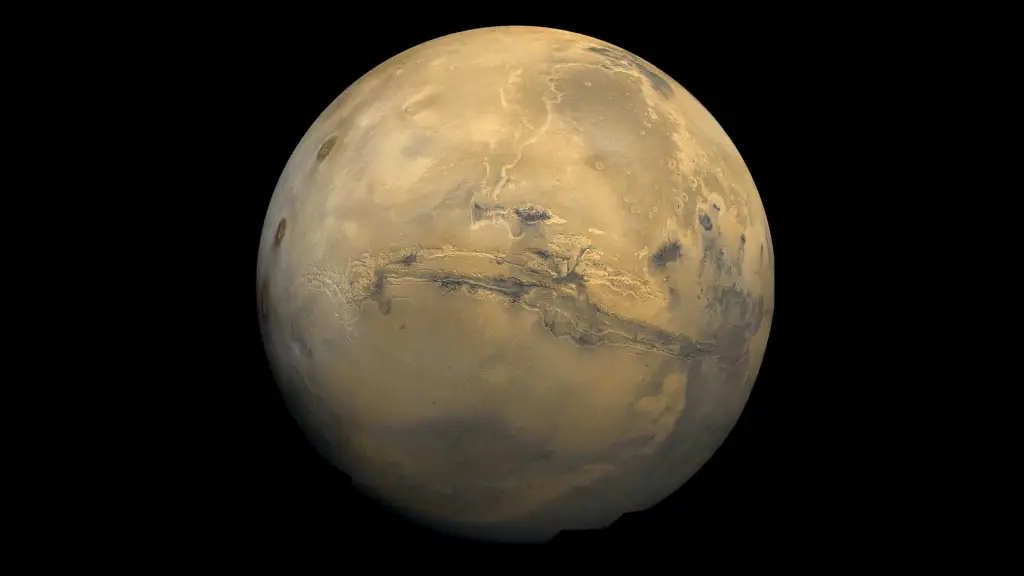
\includegraphics[width=\textwidth]{mars.png}\caption{Mars}\label{fig:mars}\end{subfigure}

    \bigskip
    {\large\textbf{Outer Planets}}\par\medskip
    \begin{subfigure}{0.22\textwidth}\centering
        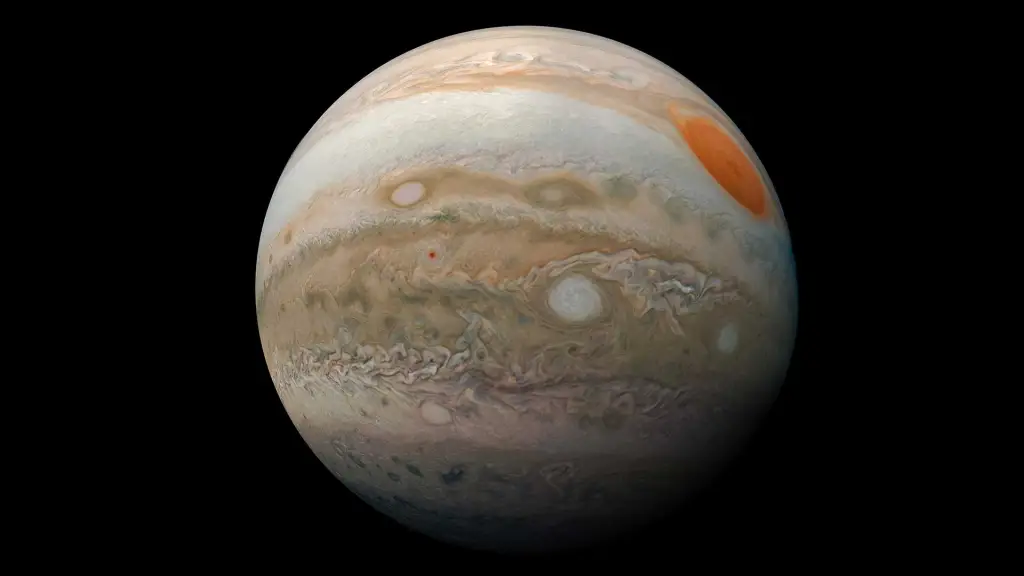
\includegraphics[width=\textwidth]{jupiter.png}\caption{Jupiter}\label{fig:jupiter}\end{subfigure}\hfill
    \begin{subfigure}{0.22\textwidth}\centering
        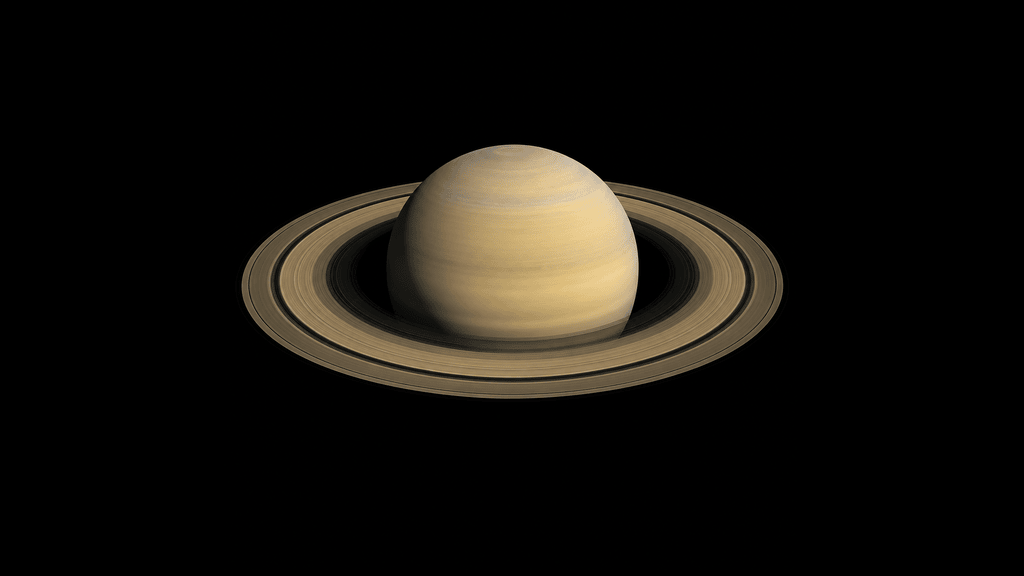
\includegraphics[width=\textwidth]{saturn.png}\caption{Saturn}\end{subfigure}\hfill
    \begin{subfigure}{0.22\textwidth}\centering
        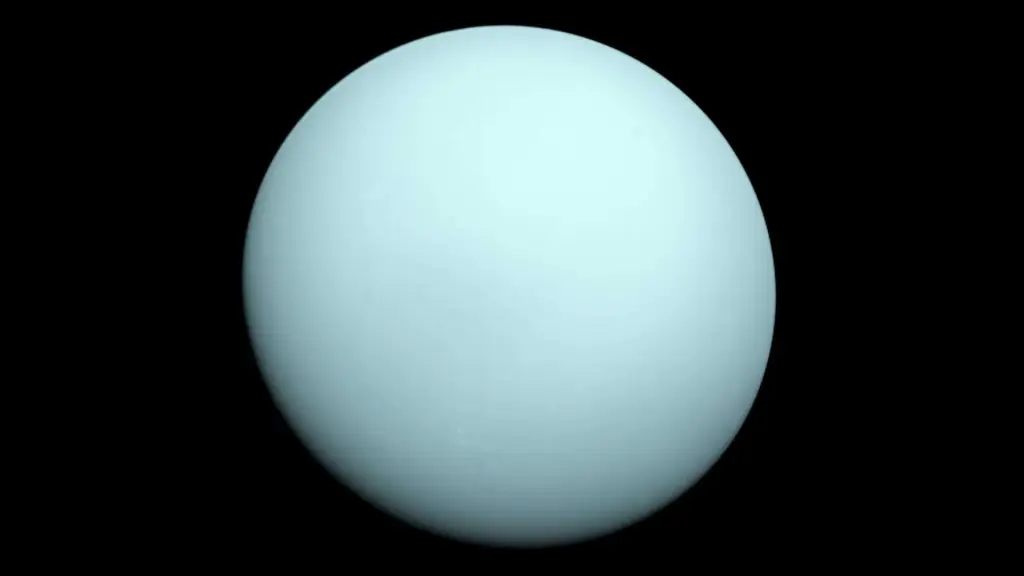
\includegraphics[width=\textwidth]{uranus.png}\caption{Uranus}\end{subfigure}\hfill
    \begin{subfigure}{0.22\textwidth}\centering
        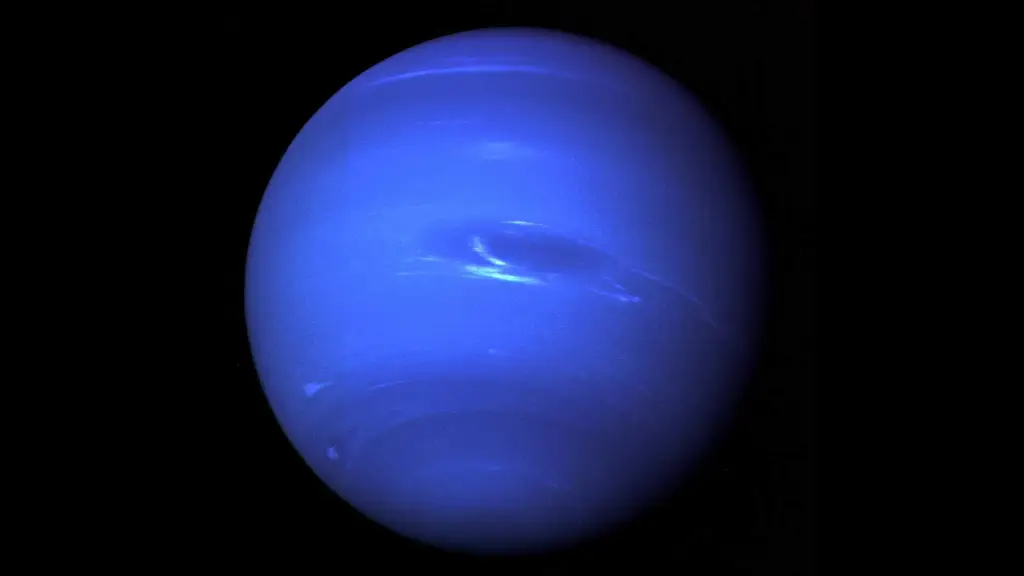
\includegraphics[width=\textwidth]{neptune.png}\caption{Neptune}\end{subfigure}
    \caption{The Sun and the eight planets of the Solar System, arranged into the
             inner and outer planetary groups. The displayed sizes and distances
             are not to scale.}
    \label{fig:solar}
\end{figure}

% ------------------------------------------------------------
\section{Kepler's Laws of Planetary Motion}
Kepler's three laws describe planetary motion~\cite{nasa_kepler}.

\subsection{First Law: Elliptical Orbits}
A planetary orbit is elliptical, with the Sun at one focus:
\begin{equation}
    \frac{x^2}{a^2} + \frac{y^2}{b^2} = 1, \qquad a \ge b > 0,
\end{equation}
Here $a$ and $b$ are the semi-axes.
For focal distance $c$,
\begin{align}
    c^2 &= a^2 - b^2 \notag \\
    e   &= \frac{c}{a}
\end{align}
Here $e$ is the eccentricity.
In polar form,
\begin{equation}\label{eq:polar}
    r(\theta) = \frac{a(1-e^2)}{1 + e\cos\theta}.
\end{equation}
Equation~\eqref{eq:polar} gives the orbital distance.

\subsection{Second Law: Equal Areas in Equal Times}
Equal times sweep equal areas:
\begin{equation}
    \Delta t_1 = \Delta t_2 \implies \Delta A_1 = \Delta A_2.
\end{equation}
Consequently, a planet moves
\begin{itemize}[label=$\diamond$]
    \item faster when it is closer to the Sun, and
    \item slower when it is farther from the Sun.
\end{itemize}

\subsection{Third Law: Orbital Period and Distance}
For planets orbiting one star,
\begin{equation}
    T^2 \propto a^3.
\end{equation}
Newtonian form:
\[
    T^2 = \frac{4\pi^2}{GM_\odot}\, a^3,
\]
Here $M_\odot$ is the solar mass.

\subsection{An Earth--Mars Comparison}
Using Earth as reference,
\[
    a_{\mathrm{E}} = 1\ \text{AU} \qquad\qquad T_{\mathrm{E}} = 1\ \text{year}
\]
where $1$ AU $\approx 1.496 \times 10^{11}$ m.\footnote{AU denotes the mean
Earth--Sun distance.} For Mars, $a_{\mathrm{M}} \approx 1.524$ AU, so
\begin{align*}
    \frac{T_{\mathrm{M}}^2}{T_{\mathrm{E}}^2}
        &= \frac{a_{\mathrm{M}}^3}{a_{\mathrm{E}}^3}, \\
    T_{\mathrm{M}}
        &= T_{\mathrm{E}}\left(\frac{a_{\mathrm{M}}}{a_{\mathrm{E}}}\right)^{3/2} \\
        &\approx (1.524)^{3/2} \approx 1.88 \text{ years.}
\end{align*}
Thus $T_{\mathrm{M}} \approx 1.88$ years.

% ------------------------------------------------------------
\section{A Relativistic Extension}
General relativity extends Kepler's model.\footnote{Planetary corrections are
small but measurable.} Einstein's equations are
\begin{equation}
    G_{\mu\nu} + \Lambda g_{\mu\nu} = \frac{8\pi G}{c^4} T_{\mu\nu}.
\end{equation}
For spherical mass $M$,
\begin{equation}
    \begin{split}
        ds^2 = {}&-\left(1 - \frac{r_s}{r}\right)c^2\,dt^2
                 + \left(1 - \frac{r_s}{r}\right)^{-1} dr^2 \\
                 &+ r^2\left(d\theta^2 + \sin^2\theta\, d\phi^2\right),
                 \qquad r_s = \frac{2GM}{c^2}.
    \end{split}
\end{equation}
Free fall satisfies
\begin{equation}
    \frac{d^2 x^\mu}{d\tau^2}
        + \Gamma^\mu_{\alpha\beta}\frac{dx^\alpha}{d\tau}\frac{dx^\beta}{d\tau} = 0.
\end{equation}
Per orbit,
\begin{equation}
    \Delta\varpi = \frac{6\pi GM}{a(1-e^2)c^2}.
\end{equation}

\begin{proposition}[Weak-field circular orbit]\label{prop:weak}
For a circular orbit of radius $r$,
\begin{equation}
    \left(\frac{v}{c}\right)^2 = \frac{GM}{rc^2} = \frac{r_s}{2r}.
\end{equation}
\end{proposition}

\begin{proof}
The circular-orbit balance $v^2/r = GM/r^2$ gives $v^2 = GM/r$. Divide by $c^2$
and use $r_s = 2GM/c^2$.
\end{proof}

See Proposition~\ref{prop:weak}.

% ------------------------------------------------------------
\section{The Outer Planets}
The outer planets are Jupiter, Saturn, Uranus, and Neptune~\cite{nasa_planets}.
The first two are \emph{gas giants}; the last two are \emph{ice giants}.
Table~\ref{tab:outer} uses scientific and relativistic notation.\footnote{Values
are rounded for typesetting practice.}

\begin{table}[ht]
    \centering
    \caption{Orbital and relativistic parameters of the outer planets}
    \label{tab:outer}
    \begin{tabular}{|c|c|c|c|c|}
        \hline
        \rowcolor{gray!15}
        \multirow{2}{*}{\textbf{Planet}}
            & \multicolumn{2}{c|}{\textbf{Orbital parameters}}
            & \multicolumn{2}{c|}{\textbf{Relativistic notation}} \\
        \cline{2-5}
        \rowcolor{gray!15}
            & $a$ (AU) & $e$ & $\varepsilon = \dfrac{1}{ac^2}GM_\odot$
            & $\beta = \sqrt{\varepsilon}$ \\
        \hline
        Jupiter & 5.204  & $4.89\times10^{-2}$ & $1.90\times10^{-9}$  & $4.36\times10^{-5}$ \\
        \hline
        Saturn  & 9.583  & $5.65\times10^{-2}$ & $1.03\times10^{-9}$  & $3.21\times10^{-5}$ \\
        \hline
        Uranus  & 19.191 & $4.72\times10^{-2}$ & $5.14\times10^{-10}$ & $2.27\times10^{-5}$ \\
        \hline
        Neptune & 30.070 & $8.6\times10^{-3}$  & $3.28\times10^{-10}$ & $1.81\times10^{-5}$ \\
        \hline
    \end{tabular}
\end{table}

Table~\ref{tab:outer} compares the four giant planets.

% ------------------------------------------------------------
%  Bibliography (IEEE-style).  The provided solar_system.bib can also be used
%  with:  \bibliographystyle{ieeetr}\bibliography{solar_system}  (run bibtex)
%  NOTE: remove the ``` fences from solar_system.bib before running bibtex.
\begin{thebibliography}{9}
\bibitem{kepler1609}
    J.~Kepler, \emph{Astronomia Nova}.\ Heidelberg, 1609.
\bibitem{nasa_kepler}
    National Aeronautics and Space Administration, ``Orbits and kepler's laws,''
    2024.
\bibitem{nasa_planets}
    National Aeronautics and Space Administration, ``About the planets,'' 2026.
    \href{https://science.nasa.gov/solar-system/}{Solar System Exploration}.
\end{thebibliography}

\end{document}
